% vim: set ai tw=80 fileencoding=utf8: 
%-------------------------------------------------------------------------------
\documentclass[
  % -- opções da classe memoir --
	12pt,				% tamanho da fonte
	openright,			% capítulos começam em pág ímpar (página vazia se preciso)
  %twoside,			% para impressão em verso e anverso. Oposto a oneside
  oneside,			% oposto de twoside, para nao gerar paginas 
	a4paper,			% tamanho do papel. 
	% -- opções da classe dc-uel --
	tcc,			% tipo do trabalho (opções: tcc, dissertacao, qualificacaoms)
	]{dc-uel}


% ---
% PACOTES
% ---

% ---
% Pacotes fundamentais 
% ---
\usepackage[T1]{fontenc}		% Selecao de codigos de fonte.
\usepackage[utf8]{inputenc}		% Codificacao do documento
\usepackage{graphicx}			% Inclusão de gráficos
% ---
		
% ---
% Pacotes adicionais, usados apenas no âmbito do Modelo Canônico do abnteX2
% ---
\usepackage{lipsum}				% para geração de dummy text
% ---

% ---
% Informações de dados para CAPA, FOLHA DE ROSTO e outros elementos
% ---
\titulo{Desenvolvimento de Técnicas de Paralelização de Código}
\tituloingles{Designing Techiniques for Code Paralellization}
\palavraschave{palavra chave1. palavra chave2.}
\palavraschaveingles{word 1. key word2.}
\autor{Luiz Guilherme Castilho Martins}
\citacaoautor{MARTINS, L. G. C.}
\data{2013}

\diadefesa{24 de novembro}
\orientador{Prof. Dr. Wesley Attrot} % É membro nato e presidente da Banca Examinadora
\membrobancadois{Prof. Dr. Segundo Membro da Banca}
\instmembrobancadois{Universidade Estadual de Londrina}
\membrobancatres{Prof. Msc. Terceiro Membro da Banca}
\instmembrobancatres{Universidade Estadual de Londrina}
% \membrobancaquatro{Prof. Esp. Quarto Membro da Banca}
% \instmembrobancaquatro{Universidade/Instituição do Quarto Membro da Banca}

% ---
% compila o indice
% ---
\makeindex
% ---

% ----
% Início do documento
% ----
\begin{document}

% Retira espaço extra obsoleto entre as frases.
\frenchspacing 

% ----------------------------------------------------------
% ELEMENTOS PRÉ-TEXTUAIS
% ----------------------------------------------------------
% \pretextual


%  % vim: set ai tw=80 fileencoding=utf8: 
%-------------------------------------------------------------------------------

\imprimircapa

%  % vim: set ai tw=80 fileencoding=utf8: 
%-------------------------------------------------------------------------------

\imprimirfolhaderosto*

\begin{fichacatalografica}
	\vspace*{\fill}					% Posição vertical
	\hrule							% Linha horizontal
	\begin{center}					% Minipage Centralizado
	\begin{minipage}[c]{12.5cm}		% Largura
	
	\imprimirautor
	
	\hspace{0.5cm} \imprimirtitulo  / \imprimirautor. --
	\imprimirlocal, \imprimirdata-
	
	\hspace{0.5cm} \pageref{LastPage} p. : il. (algumas color.) ; 30 cm.\\
	
	\hspace{0.5cm} \imprimirorientadorRotulo~\imprimirorientador\\
	
	\hspace{0.5cm}
	\parbox[t]{\textwidth}{\imprimirtipotrabalho~--~\imprimirinstituicao,
	\imprimirdata.}\\
	
	\hspace{0.5cm}
		1. Otimização.
		2. Tranformações-de-loops.
		I. Prof. Dr. Wesley Atrot.
		II\. Universidade Estadual de Londrina.\\
    %		IV\. Título\\ 			
	
	\hspace{8.75cm} CDU 02:141:005.7\\
	
	\end{minipage}
	\end{center}
	\hrule
\end{fichacatalografica}

%  % vim: set ai tw=80 fileencoding=utf8: 
%-------------------------------------------------------------------------------
\begin{errata}
Elemento opcional da% \citeonline[4.2.1.2]{NBR14724:2011}. Exemplo:

\vspace{\onelineskip}

FERRIGNO, C. R. A. \textbf{Tratamento de neoplasias ósseas apendiculares com
reimplantação de enxerto ósseo autólogo autoclavado associado ao plasma
rico em plaquetas}: estudo crítico na cirurgia de preservação de membro em
cães. 2011. 128 f. Tese (Livre-Docência) - Faculdade de Medicina Veterinária e
Zootecnia, Universidade de São Paulo, São Paulo, 2011.

\begin{table}[htb]
\center
\footnotesize
\begin{tabular}{|p{1.4cm}|p{1cm}|p{3cm}|p{3cm}|}
  \hline
   \textbf{Folha} & \textbf{Linha}  & \textbf{Onde se lê}  & \textbf{Leia-se}  \\
    \hline
    1 & 10 & auto-conclavo & autoconclavo\\
   \hline
\end{tabular}
\end{table}

\end{errata}

%  % vim: set ai tw=80 fileencoding=utf8: 
%-------------------------------------------------------------------------------

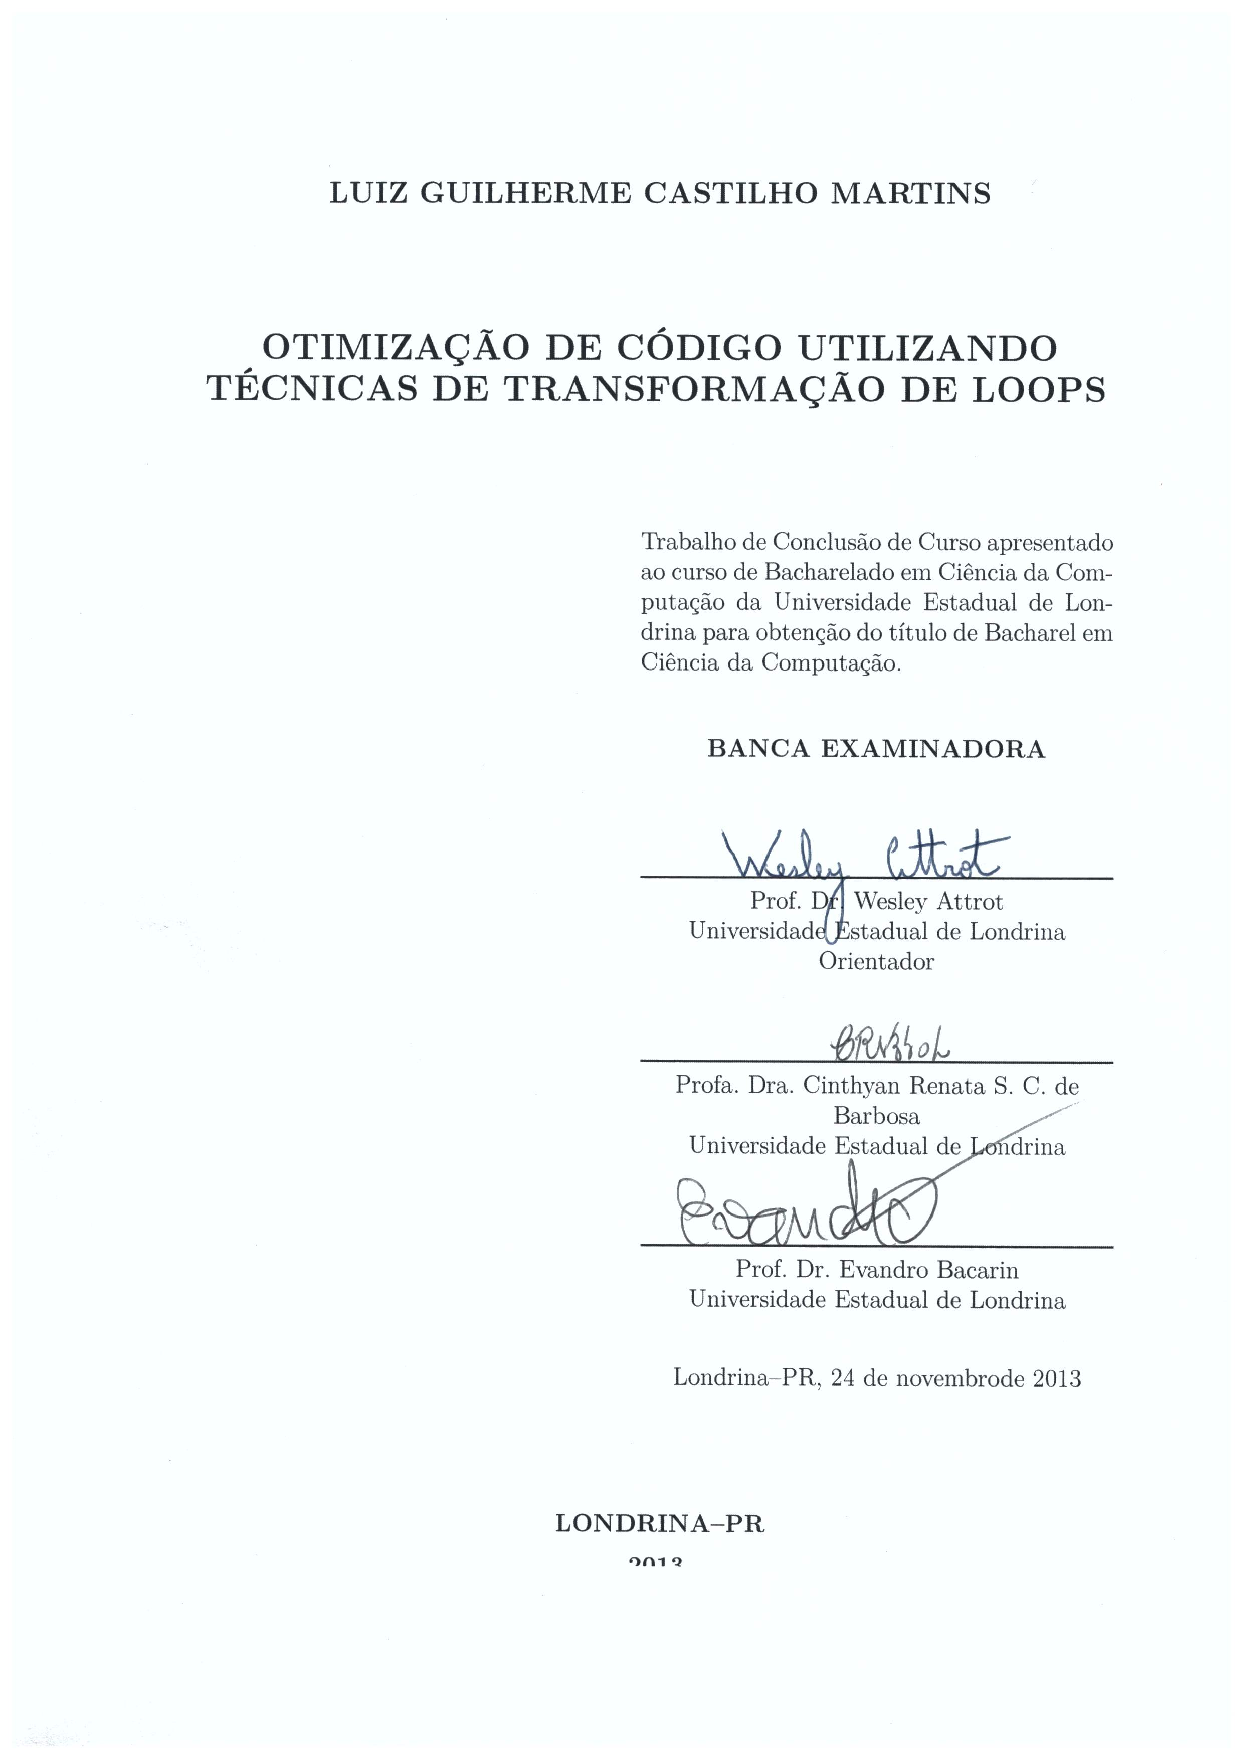
\includepdf{folha-aprovacao}

%  % vim: set ai tw=80 fileencoding=utf8: 
%-------------------------------------------------------------------------------
\begin{dedicatoria}
   \vspace*{\fill}
   \centering
   \noindent
	 \textit{A todos aqueles que \\ 
           me apoiaram e contribuíram \\ 
   para conclusão deste trabalho.} \vspace*{\fill}
\end{dedicatoria}


%  % vim: set ai tw=80 fileencoding=latin1: 
%-------------------------------------------------------------------------------

\newpage

\chapter*{AGRADECIMENTOS}

		\begin{trivlist}  \itemsep 2ex  \normalsize
					\item Agrade�o primeiramente aos meus pais por todo apoio que eles 
                me deram durante a gradua��o.
		\end{trivlist}

%  % vim: set ai tw=80 fileencoding=utf8: 
%-------------------------------------------------------------------------------
\begin{epigrafe}
    \vspace*{\fill}
	\begin{flushright}
		\textit{``O importante é ganhar. Tudo e sempre. \\
                Essa história que o importante é competir não passa de \\
                demagogia.\\
                (Ayrton Senna)}
	\end{flushright}
\end{epigrafe}

%  % vim: set ai tw=80 fileencoding=latin1: 
%-------------------------------------------------------------------------------

\newpage
\singlespacing
		\noindent MARTINS, Luiz Guilherme Castilho {\bf \titulotcc}. 2013. 
                173 f. TCC - Universidade Estadual de Londrina, 
                Londrina. 2013. \\
		\begin{center}
					{\bf {\Large RESUMO}}
		\end{center}

		\noindent Resumo.
    \newline

		\noindent{\bf Palavras-Chave:} palavra1, palavra2.

%  % vim: set ai tw=80 fileencoding=utf8: 
%-------------------------------------------------------------------------------
\begin{Abstract}
        The goal of this work is the optimization of computation of loops.
        Computationally expensive programs in general spend most of their time
        in the execution of loops.
        Loops with a large number of iterations over a big data arrays, those are
        the ones that spend of the process execution time.
        Thus, they are eligible to produce better results after optimization.
        Tecniques of loop transformation such as, loop unswitching, loop fission,
        loop fusion, loop unrolling, among others, was used in optimization.
        Analysis of data dependence was necessary to keep the meaning of the 
        program after the optimizations.
\end{Abstract}


%
%% ---
%% inserir lista de ilustrações
%% ---
%\pdfbookmark[0]{\listfigurename}{lof}
%\listoffigures*
%\cleardoublepage
%% ---
%
%% ---
%% inserir lista de tabelas
%% ---
%\pdfbookmark[0]{\listtablename}{lot}
%\listoftables*
%\cleardoublepage
%% ---
%
 % vim: set ai tw=80 fileencoding=utf8: 
%-------------------------------------------------------------------------------
\begin{siglas}
        % C
        \item[CPU] Central Processing Unit

        % D 
        \item [DFG] Data Flow Graph

        % I
        \item[IW] Instruction Word 

        % M
        \item[MISD] Multiple Instruction Single Data
        \item[MIMD] Multiple Instruction Multiple Data

        % N
        \item [NASA] National Aeronautics and Space Administration
        \item [NOWs] Network of Workstations

        % S
        \item[SISD] Single Instruction Single Data
        \item[SIMD] Single Instruction Multiple Data


        % V
        \item[VLIW] Very Long Instruction Word
\end{siglas}

%
%% vim: set ai tw=80 fileencoding=utf8: 
%-------------------------------------------------------------------------------
\begin{simbolos}
  \item[$ \delta $] Letra grega delta 
\end{simbolos}

%
%
% ---
% inserir o sumario
% ---
 \pdfbookmark[0]{\contentsname}{toc}
 \tableofcontents*
 \cleardoublepage
% ---
%
%\textual
%
%% vim: set ai tw=80 fileencoding=latin1: 
%-------------------------------------------------------------------------------
\chapter{INTRODU��O}

			%\noindent \begin{itemize}
			%			\item \indent Objetivos
			%			\item Objetivos secund�rios
			%			\item Fale sobre os objetivos do Brasil em se tornar independente tecnologicamente no desenvolvimento de microprocessadores.
			%\end{itemize}
\section{Motiva��o}
    \noindent texto.
    
\section{Objetivos e Contribui��es}

\section{Organiza��o do trabalho}

%
%% vim: set ai tw=80 fileencoding=utf8: 
%-------------------------------------------------------------------------------
\chapter{Taxonomia de Flynn}

Taxonomia de Flynn, proposta em 1966 \cite{Flynn:1966} por Michael 
Flynn e expandida em 1972 \cite{Flynn:1972}, é uma das formas de classificar o 
paralelismo disponível no processador.  

Taxonomia de Flynn utiliza o conceito de sequência de objetos ou ações, que são
chamados de \textit{stream}.
Flynn introduziu dois tipos de \textit{stream}, o 
\textit{stream} de instrução e também o \textit{stream} de dados. 

O \textit{stream} de instrução consiste em uma sequência de instruções. 
Uma instrução ou \textit{instruction word (IW)} é uma cadeia de 0's e 1's que 
representa a menor operação visível ao programador e que será executada pelo 
processador. 
Uma instrução pode conter uma ou mais operações, devido a isso
alguns autores utilizam \textit{instruction} para instruções que contenham 
apenas uma operação e \textit{instruction word} para instruções que contenham 
mais de uma operação.

\begin{comment}
Processadores escalares (\textit{scalar processors}) e processadores
superescalares (\textit{superscalar processors}) executam uma ou mais
\textit{instructions} por ciclo de \textit{clock} da máquina. 
\end{comment}

Existem no entanto quatro combinações de \textit{streams} que descrevem as 
arquiteturas de computadores mais comuns \cite{Flynn:1996}:

\begin{enumerate}
        \item \textbf{SISD:} \textit{Single Instruction, Single Data}
        \item \textbf{SIMD:} \textit{Single Instruction, Multiple Data}
        \item \textbf{MISD:} \textit{Multiple Instruction, Single Data}
        \item \textbf{MIMD:} \textit{Multiple Instruction, Multiple Data}
\end{enumerate}

Cada combinação de \textit{stream} caracteriza uma classe de arquitetura 
e cada classe possui seus tipos de paralelismo.


%-------------------------------------------------------------------------------
\section{SISD: Single Instruction, Single Data}

A classe de arquiteturas de processadores \textit{SISD}, inclui a 
maior parte dos processadores utilizados nos dias de hoje, os processadores 
\textit{single-core}, embora os programadores não percebam o paralelismo 
inerente destes processadores, muita concorrência pode estar presente.  

Em 1966 Flynn cita o \textit{Pipeline} como uma forma de se obter concorrência 
nos processadores \textit{SISD}, embora ele considere a decodificação das 
inúmeras \textit{instructions} como sendo um \textit{bottleneck}, devido a 
tecnologia da época. 
Nos dias de hoje, grande parte dos dos processadores 
utilizam-se de \textit{Pipeline} assim como também se aproveitam de alguma forma 
de múltiplas \textit{instructions}.

A concorrência em processadores \textit{SISD} são explorados durante a execução,
realizando mais de uma operação por ciclo de \textit{clock} da máquina.
%do \textit{stream} de instruções.

A quantidade e o tipo de paralelismo possível em processadores \textit{SISD}
é determinada por quatro fatores principais:

\begin{enumerate}
        \item O número de operações que podem ser executadas concorrentemente.
        \item A forma como as operações serão arranjadas para execução,
                podendo ser estaticamente, dinamicamente ou até mesmo das duas
                formas.
        \item A ordem em que as operações são colocadas e retiradas em relação
                a ordem original do programa.
        \item A maneira em o processador irá tratar cada exceção, podendo ser 
                preciso, impreciso ou das duas maneiras.
\end{enumerate}

%-------------------------------------------------------------------------------
\subsection{Processadores Escalares}

Processadores escalares são processadores simples, que executam no 
máximo uma instrução e no máximo uma operação por ciclo de \textit{clock} de 
máquina. 
As instruções do \textit{stream} de instruções são executadas 
sequencialmente, assim uma nova instrução não será executada até que a execução 
da instrução em execução seja finalizada e seu resultado devidamente
armazenado.
A semântica de instrução determina que uma sequência de ações devem ocorrer
para que se obtenha o resultado esperado, sendo: buscar a instrução,
decodifica-la, acessar o dado ou registrador, execução da operação e armazenar o
resultado. 
Podendo ocorrer \textit{overlap} entre as ações mas o resultado deve
aparecer na ordem especificada.
Esse comportamento sequencial descreve o modelo de execução sequencial.
No modelo de execução sequencial, a execução é dita \textit{instruction-precise}
se encontrar as seguintes condições:

\begin{itemize}
        \item Todas as instruções ou operações que precederam a instrução atual
                ou operação atual já foram executadas e seus resultados
                armazenados.
        \item Todas as instruções ou operações na fila de execução não foram
                executadas ou seus resultados ainda não foram armazenados.
        \item A instrução ou operação em execução no momento está em um dos
                estados de execução, tendo ou não seu resultado já armazenado.
\end{itemize}

A maioria dos processadores escalares implementam diretamente o modelo de
execução sequencial.


%-------------------------------------------------------------------------------
\subsection{Processadores Superescalares}

Enquanto processadores escalares estão limitados a executar uma única instrução 
por ciclo de \textit{clock} de máquina os processadores superescalares decoficam
várias instruções por ciclo de \textit{clock} de máquina, utilizando varios
unidades funcionais e alocação dinâmica para executar várias instruções por
ciclo de \textit{clock} de máquina. 
Processadores superescalares tem um comportamento similar ao \textit{pipeline}.

A capacidade de executar múltiplas instruções implica em verificar se existe
dependências entre as instruções, essa verificação tem que ser feita em nível de
\textit{hardware}. 
Processadores superescalares mais avançados geralmente incluem 
\textit{hardwares} que preservam a ordem e precisamente lida com as exceções, 
assim simplificando o modelo de programação.

Devido a complexidade da lógica para alocação dinâmica das instruções,
processadores superescalares de alto desempenho em geral estão limitados a
executarem de quatro a oito instruções por ciclo de \textit{clock} de máquina.


%-------------------------------------------------------------------------------
\subsection{Processadores VLIW}

Processadores VLIW (\textit{Very Long Instruction Word}) assim como os
processadores superescalares decodificam inúmeras instruções por ciclo de
\textit{clock} de máquina e utilizam várias unidades funcionais.

Ao contrário dos processadores superescalares que utilizam \textit{hardware}
para realizar alocação dinâmica das instruções os processadores VLIW executam as 
instruções através de alocação estática, essa alocação depende de uma análise do
compilador.
Assim os processadores VLIW são menos complexos e apresentam desempenho 
potencialmente maior.

Para aplicações que podem ser efetivamente alocada de forma estática os
processadores VLIW apresentam grande desempenho, embora nem todas as aplicações
tenham esta característica assim a ordem de execução estática determinada pelo
compilador não seja procedente. 
Duas classes de execução podem ocorrer e afetar o comportamento da execução 
estática:

\begin{enumerate}
        \item Atrasos de resultados de operações devido a diferença da latência
                ocorrida com a latência considerada durante a alocação pelo
                compilador.
        \item Exceções ou interrupções que colocam a ordem de execução em um
                estado não antecipado pelo compilador.
\end{enumerate}

O processador consegue lidar com os atrasos, embora isso tenha um impacto 
significante no desempenho. 
A causa mais comum de atrasos na execução devem ao dado não estar mais na 
memória cache, esse fator é tratado considerando-se o pior caso de latência 
possível e até evitando o uso da memória cache. 
Na falta de paralelismo para cobrir as lacunas da latênica, resulta na 
alocação de instruções com um número menor de operações que o processador 
consegue executar, assim diminuindo o desempenho.


%-------------------------------------------------------------------------------
\section{SIMD: Single Instruction, Multiple Data}

A classe de processadores \textit{SIMD} incluem dois tipos de
processadores, vetoriais e matriciais.
Processadores \textit{SIMD} são projetados para utilizarem determinadas
estruturas de dados, como vetores e matrizes. 
Em nível de código de máquina, programar para processadores \textit{SIMD} é 
bastante similar a processadores \textit{SISD}, a diferença é realizar operações
nas estruturas de dados agregadas. Como no processamento de algoritmos 
científicos há um grande uso de vetores e matrizes, processadores \textit{SIMD}
tem obtido grande desempenho na área.

Processadores vetoriais e matriciais apresentam diferenças tanto na 
implementação quanto na organização dos dados.

Processadores matriciais consistem em elementos de processos interconectados
cada um tendo seu próprio espaço de memória. Processadores vetoriais consistem
em um único processo que referencia a um espaço de memória global.

%-------------------------------------------------------------------------------
%\subsection{Processadores Matriciais}


%-------------------------------------------------------------------------------
%\subsection{Processadores Vetoriais}


%-------------------------------------------------------------------------------
\section{MISD: Multiple Instruction, Single Data}

A classe de processadores \textit{MISD} abstratamente é um
\textit{pipeline} de múltiplas unidades funcionais operando independentemente
sob um único \textit{stream} de dados. Em nível de micro-arquitetura é
exatamente o que os processadores vetoriais fazem.

Segundo \cite{Openshaw:1999} exceto no caso de um cientista da computação
interessado em estranhas formas de computação a classe \textit{MISD} é uma forma
restritiva e impraticável de paralelismo.

%-------------------------------------------------------------------------------
\section{MIMD: Multiple Instruction, Multiple Data}

Na classe de processadores \textit{MIMD} estão os multiprocessadores
com alguma forma de interconexão entre os processadores. Do ponto de vista do
programador, cada processo é executado independentemente e de forma cooperativa
para solucionar um mesmo problema, embora alguma forma de sincronização entre os
processos é necessária para que as informações e dados sejam trocados entre os
processadores.

Não existe limitações em que todos os processadores sejam idênticos, embora a
maioria das configurações \textit{MIMD} são homogêneos, com processadores
idênticos. Configurações heterogênias de processadores são geralmente utilizados
para aplicações com propósitos específicos.

Da perspectiva de \textit{hardware} existem dois tipos de \textit{MIMD}, sendo os
processadores \textit{multi-cores} e processadores \textit{multi-threaded}.


%-------------------------------------------------------------------------------
\subsection{Processadores Multi-Threaded}

Em \textit{multi-threaded} \textit{MIMD}, um processador base é
estendido para incluir múltiplos conjuntos de registradores para dados e para o
programa.
Com essa configuração, diferentes \textit{threads} ou programas ocupam cada
conjunto de registrador. Assim que recursos se tornam disponíveis as
\textit{threads} continuam sua execução.

Uma vez que cada \textit{thread} é independente, também o é no uso dos recursos
disponíveis, assim múltiplas \textit{threads}, fazem melhor uso dos recursos e
em consequência aumenta-se o números de instruções executadas por ciclo de
\textit{clock} de máquina.

\textit{Threads} ditas críticas, podem ter prioridade na execução para garantir
que sejam executadas em menor tempo, enquanto \textit{threads} não críticas se
utilizam de recursos ociosos.


%-------------------------------------------------------------------------------
\subsection{Processadores Multi-Core}

Os processadores \textit{multi-core} e também os múltiplos
\textit{multi-core}, necessitam comunicar os resultados de suas execuções
através a uma rede de intercomunicação e do controle de tarefas.
Assim sua implementação é significativamente mais complexa que processadores
\textit{multi-threaded}.

A rede de intercomunicação de troca dados entre os processadores e realiza a
sincronização das execuções independentes.

Quando a comunicação realizada entre os processadores através de memória
compartilhada surgem dois principais problemas, manter a consistência da memória
e também a coerência de cache.
A solução para ambos os problemas se dão em técnicas de \textit{software} e
\textit{hardware}.

%	
%% vim: set ai tw=80 fileencoding=utf8: 
%-------------------------------------------------------------------------------
\chapter{Memória}

A mais simples maneira de se melhorar o desempenho de um sistema é
replicar os computadores e criar uma forma destes trocarem dados.
Desta forma consegue-se aumentar o desempenho sem que seja necessário alterar a
\textit{CPU}.

Com o aumento contínuo da necessidade de desempenho em aplicações cada vez mais
custosas a maioria dos sistemas paralelos utilizam-se de uma entre duas
técnologias, memória distribuída ou memória compartilhada.


%-------------------------------------------------------------------------------
\section{Memória Distribuída}

Memória distribuída ou \textit{distributed memory} ou \textit{shared-nothing} é
a mais simples abordagem do ponto de vista do \textit{hardware}. 
A premissa desta abordagem é utilizar vários computadores interligados atravéz 
de uma rede.

O modelo padrão de programação consiste de processos separados para cada
computador que se comunicam atravéz da troca de mensagem ou 
\textit{message passing}, o que normalmente é feito atravéz de bibliotecas
desenvolvidas com esse propósito. 
Sendo este é o modelo mais clássico de computação paralela. 
A forma moderna de sistemas com memória distribuída iniciou a partir do trabalho 
de Seitz em 1985 \cite{Seitz:1985}.

Devido ao baixo custo de processadores voltados ao mercado consumidor e da fácil
montagem, alguns grupos exploraram tais fatores começaram a construir
\textit{cluster} de computadores pessoais. 
Tais \textit{clusters} já chamados de \textit{NOWs}, 
\textit{Network of Workstations}.
Combinando todos estes fatores com o rápido avanço de desempenho de computadores
pessoais e o avanço do \textit{open-source} junto com  versões de sistemas 
operacionais UNIX ajudaram a difundir sistemas com tais caracteristicas. 
Hoje estes sistemas são comumente conhecidos como \textit{Beowulfs} ou
\textit{Beowulf Cluster} devido ao projeto de Thomas Sterling e Donald Becker
realizado na NASA.

%-------------------------------------------------------------------------------
\section{Memória Compartilhada}

Memória compartilhada ou \textit{shared memory} é uma abordagem mais complexa, 
tornando a memória visível a todos os processadores, permitindo que 
todos possam carregar e gravar do mesmo endereço de memória. 

Entre as dificuldades desta abordagem os dois que chamam mais atenção são
coerência e consitência.
Sendo a consistência o mais problemático para o programador.




% ISA instruction set architecture

%referencias:
%sopc

%
 % vim: set ai tw=80 fileencoding=utf8: 
%-------------------------------------------------------------------------------

\section{Programação Paralela}

A programação paralela é uma camada abstrata sobre o \textit{hardware}, e em 
geral os modelos de programação paralela não são específicos para a arquitetura
de \textit{hardware}.

Existem vários modelos de programação paralela em uso na data de publicação
deste trabalho \cite{aapc}.

\begin{alineas}
        \item Memória compartilhada ou \textit{shared memory} (sem
                        \textit{threads}).
        \item \textit{Threads}.
        \item Memória distribuída ou \textit{distributed memory} (Troca de
                        mensagens ou \textit{message passing}).
        \item \textit{Data parallel}.
        \item Híbrido.
        \item SPMD (\textit{Single Program, Multiple Data}).
        \item MPMD (\textit{Multiple Program, Multiple Data}).
\end{alineas}

%-------------------------------------------------------------------------------



%
%% vim: set ai tw=80 fileencoding=utf8: 
%-------------------------------------------------------------------------------

\chapter{Data Flow Graph}

\textit{Data Flow Graph} (DFG) ou grafo de fluxo de dados, é um modelo para 
programas que expressa a possibilidade de execução concorrente de partes do
programa. 
Nos DFGs os nós representam operações (funções) e predicados a serem
aplicados a objetos de dados e as arestas representam a ligação entre o nó que
produz o dado e o nó que irá consumir aquele dado.
Na literatura os nós também são chamados de atores.
Assim, aspectos de controle e de dados de um programa podem ser representados 
em um único modelo integrado.

Embora muitas versões de DFGs tenham sido estudadas na literatura, elas possuem 
algumas características em comum:

\begin{alineas}
        \item DFG é um grafo orientado onde uma aresta é um caminho que um dado
        percorre do nó produtor para o nó consumidor.
        \item Dinamicamente, o nó de um DFG aceita um ou mais dado como entrada,
        realizando computações e devolvendo os dados do retorno para suas
        saídas.
        \item Uma ação de um nó é ativada com a presença dos dados de entrada.
\end{alineas}

Os estudos em DFGs tem sido focado principalmente em três modelos bem definidos:
DFGs estáticos, DFGs dinâmicos e DFGs síncronos.

%eopc
%-------------------------------------------------------------------------------
%\section{Subcapítulo}



%
%% vim: set ai tw=80 fileencoding=utf8: 
%-------------------------------------------------------------------------------

\chapter{Depêndencia}

Quando um programador escreve um programa em uma linguagem sequêncial, o
resultado esperado será obtido pela execução da primeira linha, depois a segundo
e assim em diante, considerando exceções de controles de fluxos como
\textit{loops} e ramificações. 
Uma vez que o programador especificou a ordem que ele espera que as computações 
sejam realizadas. 
Obter parelelismo de um programa respeitando a estas especificações não é
possível, uma vez que obter paralelismo implica em alterar a ordem das
operações realizadas.

Paralelizar um programa sequêncial significa encontrar uma ordem de execução
diferente da especificada e que irá sempre computar o mesmo resultado.
A programação sequêncial introduz restrições que podem ser críticas para o
resultado esperado do programa, assim para transformar um programa em paralelo é
importante encontrar as restrições menos críticas e realizar transformações para
que o programa continue retornando o resultado correto para qualquer entrada.

Neste capítudo serão apresentadas uma série de restrições, chamadas de
dependências que serão necessárias para garantir que as transformações
realizadas nos programas não afetem o resultado e o significado das computações
realizadas pelo programa.

Uma dependência é uma relação entre duas declarações no programa. 
Um par de declarações $<S_1,S_2>$ está em uma relação se $S_2$ é executada 
depois de $S_1$ em um programa sequêncial, e deve ser executada após $S_1$ 
em qualquer reodenação válida do programa se a ordem de acesso a 
memória será preservada.

\begin{verbatim}
S1   PI = 3.14159
S2   R = 5 
S3   AREA = PI * R * R
\end{verbatim}

Os resultados obtidos por estas declarações são definidas por aqueles obtidos
quando a ordem da execução realizada seja $<S_1,S_2,S_3>$. 
No entando nada neste trecho de código torna obrigatório a execução de 
$S_2$ depois de $S_1$, desta forma, os resultados obtidos pela ordem de execução 
$<S_2,S_1,S_3>$ serão os mesmos para a variável $AREA$ seja qual for o valor 
da entrada.
Por outro lado, o momento de execução de $S_3$ é mais crítica, se $S_3$ for
executada antes de $S_1$ ou de $S_2$, os resultados obtidos por esta execução
diferenciariam dos resultados obtidos das computações realizadas na ordem
original.
Em termos de dependência pode-se observar que os pares $<S_1,S_3>$ e $<S_2,S_3>$
estão em uma relação de dependência, embora o par $<S_1,S_2>$ não.
Dependências desse tipo são ditas dependência de dados.

Dependência em linhas de código sequêncial como visto anteriormente, é um
conceito simples de entender.
O problema é que examinar somente linhas de códigos sequênciais não garante 
eficiência em termos de paralelismo. 
Para se obter tal eficiência deve-se considerar os trechos de
código que são mais executados, ou seja devemos expandir o conceito de
dependência para \textit{loops} e vetores.
O trecho de código a seguir ilustra a complexidade introduzida ao expandirmos o
conceito de dependência.

\begin{verbatim}
        for (int I = 1; I < N; I++){
S1          A[I]   = B[I] + 1;
S2          B[I+1] = A[I] - 5;
        }
\end{verbatim}

Este \textit{loop} mostra a dependência entre $<S_1,S_2>$, uma vez que o
resultado computado de $A$ é imediatamente utilizando por $S_2$ em todas as
iterações, e também a dependêndia entre $<S_2,S_1>$ exceto na primeira iteração,
uma vez que o resultado obtido por $S_2$ será utilizado na iteração anterior.
Detectar estas dependências é difícil, considerando que cada iteração acessa 
diferentes elementos do vetor.

\textit{Loops} e vetores são apenas parte do problema que envolve a análise de
dependência, deve-se considerar também as estruturas condicionais, como as
declarações $IF$.

Deve-se no entando entender um outro tipo de dependência, dado o trecho de
código a seguir:

\begin{verbatim}
S1     if(d != 0)
S2           a = a / d;
\end{verbatim}

A declaração $S2$ não pode ser executada antes de $S1$, uma vez que essa
transformação pode ocasionar em uma divisão por zero, o que não ocorreria no
programa original. Essa dependência é chamada de dependência de controle.


%referencia: ocfma
%-------------------------------------------------------------------------------




% ----------------------------------------------------------
% ELEMENTOS PÓS-TEXTUAIS
% ----------------------------------------------------------
\postextual


% ----------------------------------------------------------
% Referências bibliográficas
% ----------------------------------------------------------
\bibliography{taxonomia-flynn/taxonomia-flynn} 

\end{document}
